\section{Result and Discussion}
\label{sec:resultdiscussion}

\subsection{Calibration Result Visualization}
\label{sec:visualisasihasil}

The visualization of the calibration results is done by comparing the data on the camera with the data on the field. This is done by entering the camera data into the \emph{Lookup Table} that has been created before. The following is the visualization of the results obtained.

\begin{figure}[ht]
  \centering
  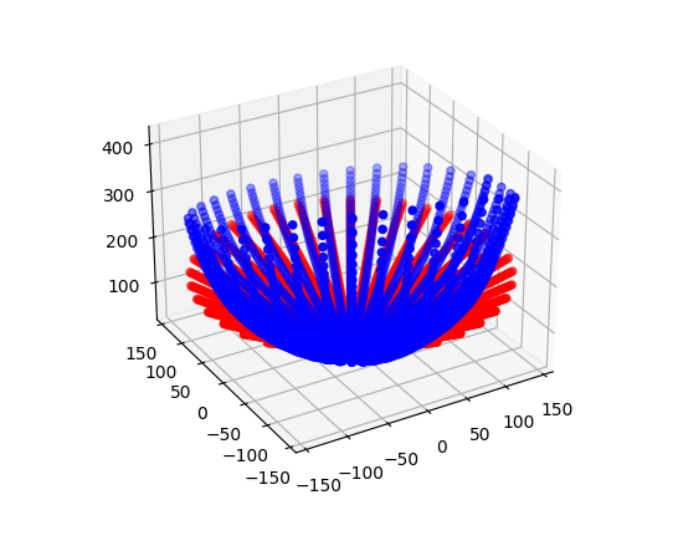
\includegraphics[width=5cm]{gambar/visual1.png}
  \caption{Visualization of calibration results.}
  \label{fig:hasilkalibrasi}
\end{figure}

From the figure above, it can be seen that the data on the camera used is not entirely projected perpendicular to the field. This happens because the camera used is not installed correctly.

\subsection{Accuracy Testing Scenario}
\label{sec:skenariopengujian}

The test is done by detecting a stationary ball on the field by rotating the robot in its position. This makes the robot able to see the ball from various angles. The test is done by taking data from the omnivision camera that has been installed on the robot and then processing the data using the \emph{Lookup Table} that has been created before so that the ball coordinates on the field are obtained. The following is the testing scenario that was carried out:

\begin{figure}[ht]
  \centering
  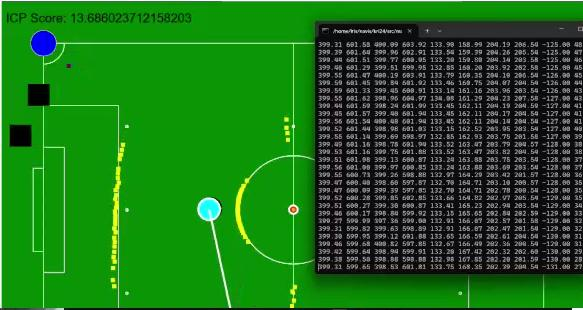
\includegraphics[width=8cm]{gambar/saat_putar_bola_2.jpeg}
  \caption{Testing Scenario.}
  \label{fig:skenariopengujian}
\end{figure}

The procedure is carried out at different distances between the robot and the ball on the field, namely at 120 cm, 200 cm, and 285 cm.

The formula used to calculate the ball's position on the field is as follows: 

\begin{equation}
  \begin{aligned}
    dx &= x\_ball\_cam - x\_center\_cam \\
    dy &= y\_center\_cam - y\_ball\_cam \\
    r\_ball\_cam &= \sqrt{dx^2 + dy^2} \\
    \theta\_ball\_cam &= \arctan(\frac{dy}{dx}) \\
    index &= \theta\_ball\_cam \times r\_max + r\_ball\_cam \\ 
    r\_ball\_fld &= r\_lookup[index] \\
    \theta\_ball\_fld &= \theta\_ball\_cam + robot\_\theta - 90 \\
    x\_ball &= robot\_x + r\_ball\_fld \times \cos(\theta\_ball\_fld) \\
    y\_ball &= robot\_y + r\_ball\_fld \times \sin(\theta\_ball\_fld) \\
  \end{aligned}
\end{equation}

\subsection{Accuracy Testing Evaluation}
\label{sec:analisispengujian}

While the test is running, the robot will rotate in its position to detect the ball on the field. The robot will rotate 30 degrees each time. The robot will rotate 12 times so that the robot can see the ball from all directions. After the robot has finished rotating, the robot will stop and the data will be recorded. The data obtained is the ball position on the field. The data is then compared with the actual ball position on the field. There are three tests that have been carried out, namely at a distance of 120 cm, 200 cm, and 285 cm. The following is the evaluation of the test results. The following data is obtained from the test results:

% Example of making a table

\begin{table}[htbp]
  \caption{Ball Position Test Results on the Field with a Distance of 120 cm.}
  \begin{center}
    \begin{tabular}{|c|c|c|}
      \hline
    \rowcolor[HTML]{C0C0C0}
  \textbf{Robot Angle to Ball} & \textbf{Ball Position X} & \textbf{Ball Position Y} \\
  \hline

  0 deg            & 407.74 cm                & 596.67 cm            \\
  30 deg           & 409.41 cm                & 600.3 cm            \\
  60 deg           & 409.65 cm                & 600.54 cm            \\
  90 deg           & 407.52 cm                & 598.2 cm           \\
  120 deg           & 407.18 cm                & 600.07 cm           \\
  150 deg           & 409.98 cm                & 598.35 cm           \\
  180 deg           & 410.66 cm                & 593.41 cm           \\
  210 deg           & 410.84 cm                & 590.28 cm           \\
  240 deg           & 410.01 cm                & 590.8 cm           \\
  270 deg           & 409.9 cm                & 594.28 cm           \\
  300 deg           & 408.91 cm                & 590.14 cm           \\
  330 deg           & 408.8 cm                & 591.57 cm           \\
  \hline
\end{tabular}
\end{center}
\end{table}

\begin{table}[htbp]
  \caption{Ball Position Test Results on the Field with a Distance of 200 cm.}
  \begin{center}

  \begin{tabular}{|c|c|c|}
  \hline
  \rowcolor[HTML]{C0C0C0}
  \textbf{Robot Angle to Ball} & \textbf{Ball Position X} & \textbf{Ball Position Y} \\
  \hline
  0 deg            & 406.44 cm                & 613.13 cm            \\
  30 deg           & 411.09 cm                & 624.66 cm            \\
  60 deg           & 416.39 cm                & 627.02 cm            \\
  90 deg           & 411.55 cm                & 625.85 cm           \\
  120 deg           & 408.85 cm                & 620.01 cm           \\
  150 deg           & 414.2 cm                & 611.7 cm           \\
  180 deg           & 415.12 cm                & 601.25 cm           \\
  210 deg           & 412.78 cm                & 592.09 cm           \\
  240 deg           & 410.77 cm                & 594.57 cm           \\
  270 deg           & 409.66 cm                & 598.43 cm           \\
  300 deg           & 407.92 cm                & 599.03 cm           \\
  330 deg           & 406.29 cm                & 602.72 cm           \\
  \hline
\end{tabular}
\end{center}
\end{table}

\begin{table}[htbp]
\caption{Ball Position Test Results on the Field with a Distance of 285 cm.}
\begin{center}

\begin{tabular}{|c|c|c|}
  \hline
  \rowcolor[HTML]{C0C0C0}
  \textbf{Robot Angle to Ball} & \textbf{Ball Position X} & \textbf{Ball Position Y} \\
  \hline
  0 deg            & 380.98 cm                & 593.81 cm            \\
  30 deg           & 382.14 cm                & 594.49 cm            \\
  60 deg           & 383.41 cm                & 607.18 cm            \\
  90 deg           & 392.49 cm                & 604.67 cm           \\
  120 deg           & 390.32 cm                & 606.04 cm           \\
  150 deg           & 391.43 cm                & 598.47 cm           \\
  180 deg           & 387.17 cm                & 587.89 cm           \\
  210 deg           & 390.16 cm                & 577.15 cm           \\
  240 deg           & 389.67 cm                & 585.82 cm           \\
  270 deg           & 389.38 cm                & 590.31 cm           \\
  300 deg           & 382.61 cm                & 593.25 cm           \\
  330 deg           & 380.73 cm                & 589.31 cm           \\
  \hline
\end{tabular}
\end{center}
\end{table}

Each table contains the ball position data on the field at different distances. Every data in that table is the ball position data on the field at a certain angle. The data is then compared with the actual ball position on the field. The comparison is done by calculating the standard deviation of the data obtained. The formula used to calculate the standard deviation is as follows: 

\begin{equation}
  \begin{aligned}
    \sigma &= \sqrt{\frac{\sum_{i=1}^{n} (x_i - \bar{x})^2}{n}} \\ 
  \end{aligned}
\end{equation}

Where $\sigma$ is the standard deviation, $x_i$ is the data, $\bar{x}$ is the average of the data, and $n$ is the number of data.

From the table, the standard deviation in the ball position data on the field with a distance of 120 cm is 1.26 cm and 4.11 cm for the ball position x and y. Meanwhile, at a distance of 200 cm, the standard deviation is 3.28 cm and 12.80 cm for the ball position x and y. At a distance of 285 cm, the standard deviation is 4.40 cm and 8.92 cm for the ball position x and y. 

From these results, it can be concluded that the calibration system that has been created can detect the ball position on the field well. The ball not being exactly in the middle of the field can be caused by several factors. Some of the factors causing this are the inaccuracy of the ball position in the real world, the inaccuracy of the robot position in the real world, and the inaccuracy of the robot orientation in the real world. Because basically according to the formula \textbf{4.1}, the ball position on the field is also determined by the robot's position on the field.

\subsection{Second Accuracy Testing Scenario}
\label{sec:skenariopengujian2}

The second accuracy test is by comparing the new calibration results with the old calibration that still uses the \emph{polynomial regression} algorithm. The test is done in the same way as the previous accuracy test. However, the calculation process uses the \emph{polynomial regression} algorithm.

\subsection{Second Accuracy Testing Evaluation}
\label{sec:analisispengujian2}

The test is done by comparing the data obtained from the new calibration with the data obtained from the old calibration. The following is the data obtained from the test results: 

\begin{table}[htbp]

\caption{Ball Position Test Results on the Field with a Distance of 120 cm using the Old Calibration.}
\begin{center}

\begin{tabular}{|c|c|c|}
  \hline
  \rowcolor[HTML]{C0C0C0}
  \textbf{Robot Angle to Ball} & \textbf{Ball Position X} & \textbf{Ball Position Y} \\
  \hline
  0 deg            & 370.18 cm                & 576.31 cm            \\
  30 deg           & 376.24 cm                & 585.42 cm            \\
  60 deg           & 383.91 cm                & 597.98 cm            \\
  90 deg           & 392.99 cm                & 605.67 cm           \\
  120 deg           & 390.23 cm                & 610.94 cm           \\
  150 deg           & 400.49 cm                & 598.89 cm           \\
  180 deg           & 385.97 cm                & 582.89 cm           \\
  210 deg           & 398.61 cm                & 577.15 cm           \\
  240 deg           & 390.76 cm                & 585.02 cm           \\
  270 deg           & 386.32 cm                & 588.91 cm           \\
  300 deg           & 378.69 cm                & 585.55 cm           \\
  330 deg           & 370.32 cm                & 579.11 cm           \\
  \hline
\end{tabular}
\end{center}
\end{table}

From the data, it can be seen that the standard deviation in the ball position data on the field with a distance of 120 cm using the old calibration is 10.01 cm and 11.32 cm for the ball position x and y. Meanwhile, in the new calibration, the standard deviation is 1.26 cm and 4.11 cm for the ball position x and y. It can be seen that the new calibration is better than the old calibration. This happens because the camera is not installed correctly on the robot, causing the old calibration results to be inaccurate. The inaccuracy occurs because the old calibration only uses one direction as a reference for the polynomial regression model. Whereas, in reality, the model formula for each camera direction will always be different.

\subsection{Third Accuracy Testing}
\label{sec:skenariopengujian3}

The third accuracy test is placing robot somewhere on the field and then the robot will see lines around the robot. The robot will detect each pixel of line and then the robot will calculate the distance between the robot and the line. So the robot can visualize the line on the field. The test is done by taking data from the omnivision camera that has been installed on the robot and then processing the data using the \emph{Lookup Table} that has been created before so that the line coordinates on the field are obtained. The following is the testing scenario that was carried out: 

\begin{figure}[htbp]
  \centering
  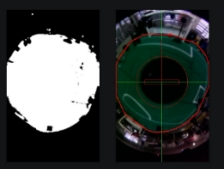
\includegraphics[width=7cm]{gambar/cam_raw1.jpg}
  \caption{Raw frame.}
  \label{fig:skenariopengujian31}
\end{figure}

The left picture is the field binary image that calculated to get the line binary image. 

\begin{figure}[htbp]
  \centering
  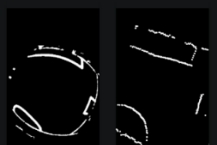
\includegraphics[width=7cm]{gambar/cam_raw2.jpg}
  \caption{Calculated frame.}
  \label{fig:skenariopengujian32}
\end{figure}

The left picture is the line binary image that calculated to get the line coordinates on frame. Extracting the line coordinates on the frame is done by scanning from the center of frame to the edge of frame.  

\begin{algorithm}[htbp]
  \caption{Process Lines on Frame}\label{alg:process_lines}
  \begin{algorithmic}[1]
  \Procedure{ProcessLinesOnFrame}{}
      \State \text{Initialize lines\_on\_frame as an empty vector}
      \For{\text{angle from 0 to 360 with step size 2.5}}
          \State \text{Initialize dist to 0}
          \For{\text{index from 0 to 320}}
              \State $x \gets \text{dist} \times \cos(\text{angle}) + \text{center\_cam\_x}$
              \State $y \gets \text{center\_cam\_y} - \text{dist} \times \sin(\text{angle})$
              \If{\text{frame[y][x] == 255}}
                  \State \text{Push (x, y) to lines\_on\_frame}
              \EndIf
              \State $dist \gets \text{dist} + 1$
          \EndFor
      \EndFor
  \EndProcedure
  \end{algorithmic}
\end{algorithm}

% Dummy
After getting the line coordinates on the frame, the robot will calculate the world coordinates of the line. The formula used to calculate the line's position on the field is as follows:

\begin{equation}
  \begin{aligned}
    dx &= x\_line\_cam - x\_center\_cam \\
    dy &= y\_center\_cam - y\_line\_cam \\
    r\_line\_cam &= \sqrt{dx^2 + dy^2} \\
    \theta\_line\_cam &= \arctan(\frac{dy}{dx}) \\
    index &= \theta\_line\_cam \times r\_max + r\_line\_cam \\ 
    r\_line\_fld &= r\_lookup[index] \\
    \theta\_line\_fld &= \theta\_line\_cam + robot\_\theta - 90 \\
    x\_line &= robot\_x + r\_line\_fld \times \cos(\theta\_line\_fld) \\
    y\_line &= robot\_y + r\_line\_fld \times \sin(\theta\_line\_fld) \\
  \end{aligned}
\end{equation}

After the robot has finished calculating the line's position on the field, the robot will visualize the line on the field. The visualization can be seen on right picture of figure \ref{fig:skenariopengujian32}.


\subsection{Computational Speed Testing Scenario}
\label{sec:analisispengujian}

The test is done by comparing whether the new calibration system is faster than using the old calibration system. The test is done by recording the time after calibration and subtracting it from the time before calibration. So that an estimate of the time it takes for the system to perform the calculation process for calibration can be obtained. The following formula is used to calculate the delay time:

\begin{equation}
  \begin{aligned}
    delay\_time &= time1 - time0 \\ 
  \end{aligned}
\end{equation}

Where $time1$ is the time after calibration and $time0$ is the time before calibration.

\subsection{Computational Speed Testing Evaluation}
\label{sec:analisispengujian}

From the tests that have been carried out, there are 10 iterations that have been done. The following is the data obtained from the test results:

\begin{table}[htpb]
  \caption{Difference in Computational Speed Test Results}
\begin{center}

\begin{tabular}{|c|c|c|}
  \hline
  \rowcolor[HTML]{C0C0C0}
  \textbf{Iteration to-} & \textbf{New Calibration Time} & \textbf{Old Calibration Time} \\
  \hline
  0            & 119 ns                & 176 ns            \\
  1           & 76 ns                & 86 ns            \\
  2           & 25 ns                & 107 ns            \\
  3           & 31 ns                & 90 ns           \\
  4           & 32 ns                & 88 ns           \\
  5           & 36 ns                & 87 ns           \\
  6           & 37 ns                & 88 ns           \\
  7           & 34 ns                & 93 ns           \\
  8           & 37 ns                & 89 ns           \\
  9           & 35 ns                & 90 ns           \\
  \hline
\end{tabular}
\end{center}
\end{table}

From the graph, it can be seen that the new calibration system is 53.2 ns faster than the old calibration system. With an average of 46.2 ns for the new calibration and 99.4 ns for the old calibration. This is because the new calibration system only uses a \emph{Lookup Table} containing camera calibration data. Whereas the old calibration system uses the polynomial regression algorithm which takes longer.


